\subsection{Valid and Invalid Arguments}
\hrulefill

\paragraph*{Definition}
An \textbf{argument} is a sequence of statements, and an \textbf{argument form} is a sequence of statement form.

\begin{itemize}
    \item The final statement or statement form is called the \textbf{conclusion}. The symbol $\therefore$ (therefore) is used to denote the conclusion.
    \item All the preceding statements or statement forms are called \textbf{premises}, or assumptions or hypotheses.
    \item An argument form is \textbf{valid} means if all premises are true, then the conclusion must also be true.
\end{itemize}

\paragraph*{Example}
Determine whether the following argument form is valid or invalid:
\begin{align*}
    p &\implies q \lor \neg r\\
    q &\implies p \land r\\
    \therefore p &\implies r
\end{align*}
\begin{center}
    \begin{tabular}{|c|c|c|c|c|c|c|}
        \hline
        $p$ & $q$ & $r$ & $p \implies (q \lor \neg r)$ & $q \implies (p \land r)$ & $p \implies r$ & Valid?\\
        \hline
        T & T & T & T & T & T & Valid\\
        T & T & F & F & T & F & Invalid\\
        T & F & T & T & F & T & Invalid\\
        T & F & F & F & F & F & Invalid\\
        F & T & T & T & F & T & Invalid\\
        F & T & F & T & F & T & Invalid\\
        F & F & T & T & F & T & Invalid\\
        F & F & F & T & F & T & Invalid\\
        \hline
    \end{tabular}
\end{center}
Therefore the argument form is invalid.

\pagebreak

\subsubsection*{Syllogisms}
\paragraph*{Definition}
An argument form with two premisies are called syllogism. The firest and second premises are called the 
major premise and minor premise respectively.

\paragraph*{Modus Ponens}
Modus Ponens is a valid argument form that can be expressed as:
\begin{align*}
    p &\implies q\\
    p &\\
    \therefore q &
\end{align*}

This means that if $p \implies q$ (if $p$ then $q$) is true, and $p$ is true, then we can conclude that $q$ must also be true.
\paragraph*{Example}
If there are more pigeons than there are pigeonholes, then at least two pigeons roost in the same hole.\\
There are more pigeons than there are pigeonholes.\\
$\therefore$ At least two pigeons roost in the same hole.

\paragraph*{Modus Tollens}
Modus Tollens is a valid argument form that can be expressed as:
\begin{align*}
    p &\implies q\\
    \neg q &\\
    \therefore \neg p &
\end{align*}

This means that if $p \implies q$ (if $p$ then $q$) is true, and $q$ is false, then we can conclude that $p$ must also be false.

\pagebreak

\paragraph*{Rules of Inference}
A rule of inference is a form of argument that is valid. Both modus ponens and modus tollens are rules of inference. The following 
are additional examples of rules of inference:
\begin{center}
    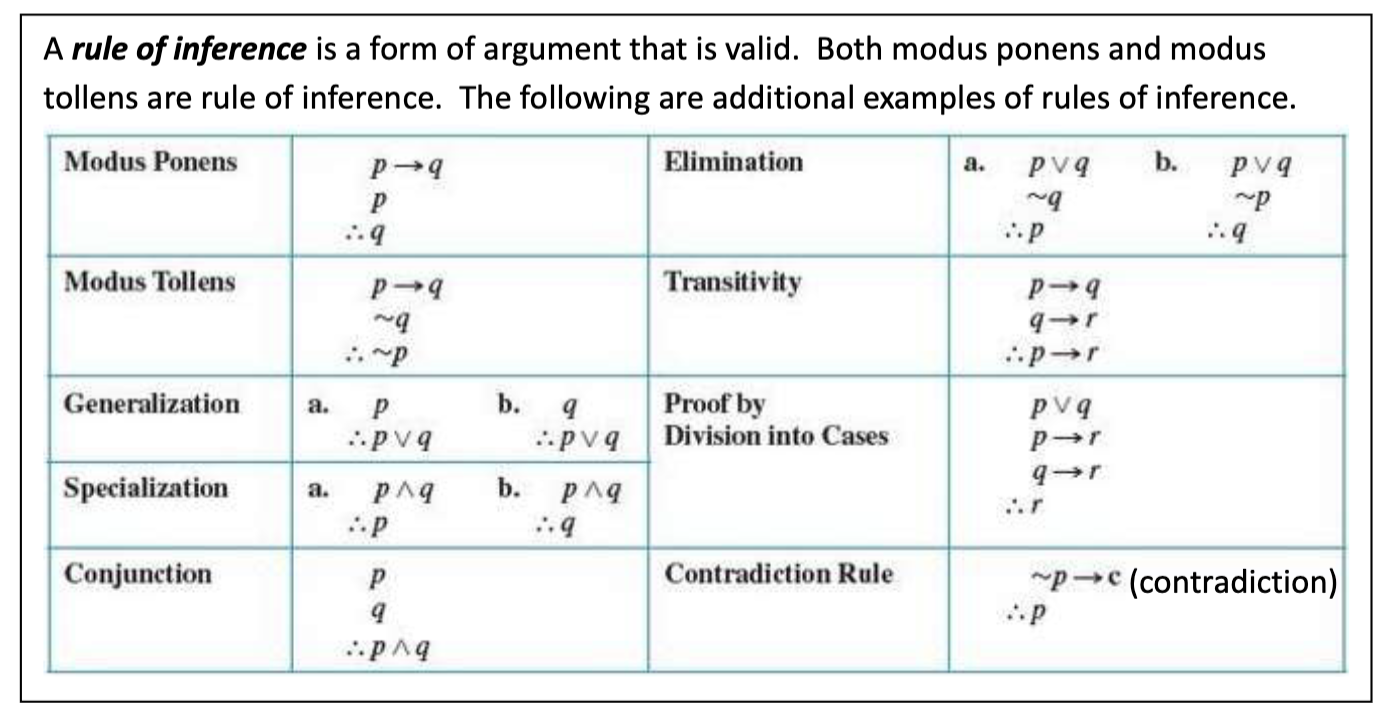
\includegraphics[width=0.75\textwidth]{rule-of-inference.png}
\end{center}

\begin{align*}
    \text{Prove by Detachment} \\
    \text{Prove by contrapositive}\\
    \text{Disjunctive of syllogism}\\
    \text{Law of Syllogism}\\
\end{align*}

\subsubsection*{Contradictions}
\paragraph*{Definition}
A contradiction is a statement that is always false.
\begin{align*}
    &\neg p \implies c\\
    &\therefore p
\end{align*}
\pagebreak
\paragraph*{2 column rule}
The 2 column rule is a way to prove by contradiction. For example with knights and knaves. Knights always
tell the truth and knaves always lie:
\begin{itemize}
    \item A says B is a knight
    \item B says A and I are of opposite types
\end{itemize}

\hrulefill\\

Suppose A is a knight:
\begin{center}
    \begin{tabular}{c|c}
    \hline
    What A says must be true & By the definition of a knight\\
    \hline
    B is a knight & by given (what A says)\\
    \hline
    What B says must be true & By the definition of a knight\\
    \hline
    A and B are of opposite types & by given (what B says)\\
    \hline
    Contradiction & A is not a knight or A is a knave\\
    \hline
    The supposition is false & by rule of contradiction\\
    \hline
    A is not a knight or A is a knave & by negation of supposition.\\
    \hline
    \end{tabular}
\end{center}